Metoda macierzy przejścia, w skróce nazywana TMM (ang. transfer matrix method) jest używana w optyce i akustyce do analizy propagacji fal odpowiednio elektromagnetycznych i dzwiękowych przez ośrodki warstwowe. Metoda macierzy przejścia może być wykorzystywana do modelowania współczynników transmisji i odbicia w układach liniowych niezmienniczych ze wzlgędu na przesunięcia w kierunku prostopadłym do granicy ośrodków.

W elektromagnetyzmie, macierz przejścia dowolnego układu optycznego wiąże ze sobą amplitudy pól padających i wychodzących \cite{teich1991fundamentals,markos2008wave}:
\begin{equation}
\begin{bmatrix}
U_i \\ 
U_r
\end{bmatrix}
= M 
\begin{bmatrix}
U_t \\
U_b
\end{bmatrix},
\label{eq:tmm}
\end{equation}
gdzie $M$ jest macierzą przejścia układu, $U$ jedt dowolną wybraną skłądową pola elektrycznego lub magnetycznego, odpowiednio $U_i$ - padającą, $U_r$ - odbitą, $U_t$ - transmitowaną przez układ, oraz $U_b$ padającą  z przeciwnej strony. Graficznie sytuację opisywaną powyższym równaniem przedstawia schemat na rysunku \ref{fig:tmm-simple}.

\begin{SCfigure}
	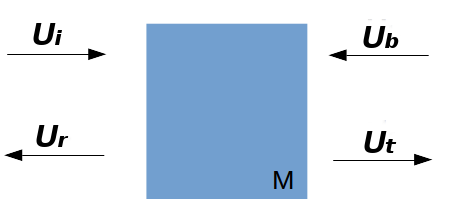
\includegraphics[width=0.6\textwidth]{images/tmm.png}
	\caption{Ilustracja podstawowego elemntu w symulacjach metodą TMM, wraz z ilustracją amplitud z równanie (\ref{eq:tmm}) }
	\label{fig:tmm-simple}
\end{SCfigure}

W przypadku analizy układu złożonego z wielu warstw, oznaczenia z wzoru (\ref{eq:tmm}), możemy poprzez indeks liczbowy przypisać osobno do każdej z macierzy $M_i$:
\begin{equation}
\begin{bmatrix}
U_i^1 \\ 
U_r^1
\end{bmatrix}
= M_1 
\begin{bmatrix}
U_t^1 \\
U_b^1
\end{bmatrix},
\label{eq:tmm-1l}
\end{equation}

\begin{equation}
	\begin{bmatrix}
	U_i^2 \\ 
	U_r^2
	\end{bmatrix}
	= M_2 
	\begin{bmatrix}
	U_t^2 \\
	U_b^2
	\end{bmatrix},
\label{eq:tmm-2l}
\end{equation}

dodając kolejne warstwy np. po lewej stronie od warstwy z rysunku \ref{fig:tmm-simple}, wtedy obliczone $U_i^1$ i $U_r^1$ według wzoru \ref{eq:tmm-1l} dla kolejnej warstwy mają znacznie odpowiednio $U_t^2$ i $U_b^2$. Podstawiając to do wzoru \ref{eq:tmm-2l} otrzymujemy 
\begin{equation}
\begin{bmatrix}
U_i^2 \\ 
U_r^2
\end{bmatrix}
=M_2 M_1 
\begin{bmatrix}
U_t^1 \\
U_b^1
\end{bmatrix},
\label{eq:tmm-2ls}
\end{equation}

Z czego wynika, że w układ złożony z i warstw opisywanych macierzami przejscia $M_i$ można traktować jak jeden element opisywany przy pomocy macierzy przejścia będącej iloczynem macierzy opisujących wszystkie jego elementy $M= M_i \cdot M_{i-1} ... \cdot M_1$. Podstawowymi macierzami przejścia wykorzystywanymi do obliczeń w układach warstwowych są
\begin{itemize}
\item Macierz przejścia odpowiadająca propagacji w ośrodku jednorodnym 
\begin{equation}
	M_p=
	\begin{bmatrix}
	\textrm{exp}(-2i\pi k z_0) & 0 \\
	0	&\textrm{exp}(-2i\pi k z_0)\\
	\end{bmatrix},gdzie
\end{equation}
$k$ jest długością wektora falowego w ośrodku w którym zachodzi propagacja w kierunku równoległym do grubości warstwy, a $z_0$ jest grubością warstwy.
\item Macierz opisująca przejście fali E-M przez granicę ośrodków
\begin{equation}
	M_i=\frac{1}{1+r}
	\begin{bmatrix}
	1 & r \\
	r & 1\\
	\end{bmatrix},
\end{equation}
gdzie $r$ jest amplitudowym współczynnikiem odbicia fali na opisywanej granicy ośrodków wynikającym z równań Fresnela i zależnym od kąta padania. 
\end{itemize}

Obliczenie współczynnika transmisji płytki płasko-równoległej wymaga więc skonstruowania macierzy opisującej taką płytkę z trzech macierzy: 
\[
M=M_i \cdot M_p \cdot  M_i.
\]
